% !TEX encoding = UTF-8 Unicode
% !BIB TS-program = biber 
% !BIB program = biber    

% This file is MIT-Thesis.tex, a LaTeX template for formatting an MIT thesis with the mitthesis class.
%
% Version: 1.11, 2023/11/02
%
% Author: John H. Lienhard, copyright 2023. Reuse under the MIT license: https://ctan.org/license/mit 

% Documentation is here: https://ctan.org/pkg/mitthesis

%% Don't modify the \DocumentMetadata command unless you know what it does. 
%% If this command throws an "undefined" error, your latex system is out of date: try commenting this command out.
% \DocumentMetadata{ 
% 	pdfstandard = a-2b,
% 	pdfversion  = 1.7,
% 	lang		= en-US,
% %	debug		= {xmp-export}, % uncomment to output a separate xmpi file showing the metadata
% }
%%%%%%%%%%%%%%%%%%%%%%%%%%%%%%%%%%%%%%%

% This file was adapted from MIT thesis to be used
% by the University of Massachusetts Lowell
% Modified by: Monish Reddy Kotturu

\documentclass[fontset=newtx]{mitthesis} %,fontset=libertine, fontset=newtx-sans-text, fontset=heros-stix2, fontset=stix2
%
% option [twoside]		gives facing-page behavior for printing; omitting twoside will eliminate even-numbered blank pages.
% option [lineno]	 	provides line numbers, as for editing
% option [mydesign] 	loads packages for color, title and list formats, margins, or captions: edit mydesign.tex to change defaults.
% option [fontset] is a keyvalue which can be:
%					 	pdftex or unicode engines:  defaultfonts, libertine, lucida
%					 	pdftex only: 				fira-newtxsf, newtx, newtx-sans-text
%						unicode engines (luatex):	heros-stix2, stix2, termes, termes-stix2
%					 	if no key value is given, fonts default to CMR (pdftex) or LMR (unicode), i.e., "the LaTeX font".
%					 	You can edit the fontset files or you can write your own, myfonts.tex, and do [fontset=myfonts].
%						If you are using multiple languages, load the babel package in your fontset file, before the fonts.

%%%%%%%%% Packages used in sample chapters (not otherwise required) %%%%%%%

%% Package for code listing in Appendix A.
\usepackage{listings}%   documentation is here https://ctan.org/pkg/listings

%% Set chemical formulas nicely
\usepackage[version=4]{mhchem}%   documentation is here https://ctan.org/pkg/mhchem

%% Latin filler used in Chapter 1, with a test for package version date. https://ctan.org/pkg/lipsum
\usepackage{lipsum}
\IfPackageAtLeastTF{lipsum}{2021/09/20}{\setlipsum{auto-lang=false}}{}


%%%%%%%%%  Graphics path (to figure files)  %%%%%%%%%%%%%%%%%%%%%%%%%%%%%%%%

%% Can set graphicspath to point to specific directories containing figures (the current directory is searched automatically)
%% For instance, to search a subdirectory of the current directory called "figures" and a parallel directory called "art", set:

% \graphicspath{ {figures/} {../art/} }% For details see: https://latexref.xyz/dev/latex2e.html#g_t_005cgraphicspath


%%%%%%%%%  Representative set-up for biblatex  %%%%%%%%%%%%%%%%%%%%%%%%%%%%%

\usepackage[style=ieee,maxbibnames=10,sorting=none]{biblatex}% style=ext-numeric-comp,articlein=false,giveninits=true
	\DefineBibliographyStrings{english}{url= \textsc{url} ,  }% replaces default "[Online]. Available" by "URL"


\addbibresource{citations.bib}%% <== change to YOUR bib file <= CHANGE

%% to avoid split urls and stretched white space, you can set the bibliography ragged-right:
%\appto{\bibsetup}{\raggedright}

% biblatex is very powerful, and you can customize most aspects the reference list and citations to suit your needs.
% documentation is here: https://ctan.org/pkg/biblatex


%%%%%%%%%%  Option to use natbib   %%%%%%%%%%%%%%%%%%%%%%%%%%%%%%%%%%%%%%%%%

%\RequirePackage[numbers,sort&compress]{natbib}
 
%%% add bibliography to table of contents
%\apptocmd{\bibliography}{\addcontentsline{toc}{chapter}{\protect\textbf{\bibname}}}{}{}

%%% You can use this to rename the bibliography section
%\renewcommand{\bibname}{References}

%%% Can adjust space between bibliography items (change 4pt to something else; don't drop last two lengths, they are stretchable "glue")
%\setlength\bibsep{4pt plus 1pt minus 1pt}


%%%%%%%%%%  Table related packages  %%%%%%%%%%%%%%%%%%%%%%%%%%%%%%%%%%%%%%%%

\usepackage{booktabs}% better quality tables, https://ctan.org/pkg/booktabs
\usepackage{array}%    additional options for table columns, https://ctan.org/pkg/array

%\usepackage{tabularx}%   https://ctan.org/pkg/tabularx

%\usepackage{dcolumn}%    alignment on decimal place, https://ctan.org/pkg/dcolumn
%\newcolumntype{d}[1]{D{.}{.}{#1}}


%%%%%%%%%%  Option for "double spacing" %%%%%%%%%%%%%%%%%%%%%%%%%%%%%%%%%%%%

%% Back in the typewriter era, double spaced lines were convenient for editing with a pencil. 
%% In typography, the separation between lines is called "leading", and it is usually set in 
%% proportion to the font size (i.e., when the font is loaded).  If you really feel the need 
%% to change the line separation, the most attractive results will be obtained by changing the
%% leading in proportion to the the current font size, rather than just doubling the space.

%% The setspace package provides a tool for changing line separation. Use these two commands here:
%
\usepackage{setspace}%  documentation at https://ctan.org/pkg/setspace
% \setstretch{1.1}% you can choose some other value for the stretch of space between lines
%
%% Use one or more of the these commands AFTER the frontmatter
%
% \onehalfspacing
% \doublespacing
% \singlespacing  % will turn these effects off (you can use these anywhere in the document)

%% The best result may be to stay with leading selected by the typographer who set up the font.


%%%%%%%%%%%  Metadata  %%%%%%%%%%%%%%%%%%%%%%%%%%%%%%%%%%%%%%%%%%%%%%%%%%%%%%%

% Most of the document metadata is created automatically. 
% The following items should be adjusted to match your work. <================= !!!!!!!!!!

\hypersetup{%
	pdfsubject={Template for writing MIT theses with the mitthesis class},
	% Change this to briefly state topic of your thesis 
% 
	pdfkeywords={University of Massachusetts Lowell, UML},
	% Add keywords that will help search engines and libraries to find your work.
	% Includes the name[s] of the author[s] 
	% (If you have used \DocumentMetadata, at line 15, you can just put "\CopyrightAuthor," for the names.)
%
	pdfurl={},
	% If you have a url for the thesis, put it here. Otherwise delete this.
	% (MIT Libraries will put your thesis in DSPACE with a persistent url after you submit it.)
%	
	pdfcontactemail={},
	% You can put a [permanent] email address into the metadata, if you like.
	% Otherwise delete this.
%
	pdfauthortitle={},
	% If you have a title, you can include it here.
}

%%%%%%%%%%%%%%  End preamble %%%%%%%%%%%%%%%%%%%%%%%%%%%%%%%%%%%%%%%%%%%%%%%%%%%%%%%%%%%%%%%%%%%%%
%%%%%%%%%%%%%%%%%%%%%%%%%%%%%%%%%%%%%%%%%%%%%%%%%%%%%%%%%%%%%%%%%%%%%%%%%%%%%%%%%%%%%%%%%%%%%%%%%%

%% my commands and packages%%
\usepackage{newtxtext, newtxmath}
\usepackage{graphicx}

\newcommand{\attn}[1]{\textcolor{red}{#1}}

\Institution{University of Massachusetts Lowell}

\begin{document}

%%% edit the following commands to match your thesis %%%%%%%%%%

\title{THESIS TITLE}

% \Author{Author full name}{Author department}[Author's first PREVIOUS degree][Author's second PREVIOUS degree][...
% Note that third, fourth, fifth, and sixth arguments are optional [] and may be omitted

% note on names: most of the following names are made up; Silas Holman was a physics professor at MIT in the 19th century.

\Author{Author Name}{Department}

% Use once for each degree fulfilled by thesis
% For two degrees from one department, leave the department argument blank for the second degree {}.
% \Degree{Bachelor of Science in Physics}{Department of Physics}
% \Degree{Master of Science in Physics}{}
\Degree{Degree}{Department}

% If there is more than one supervisor, use the \Supervisor command for each.
\Supervisor{Supervisor}{Department}
\CommitteeMember{Committee Member}{Department}
\CommitteeMember{Committee Member}{Department}

% Professor who formally accepts theses for your department (e.g., the Graduate Officer, Professor Sméagol,...)
% If more than one department, use more than once
% **If you need to reduce vertical space, put the acceptor title in the second argument and leave the third blank {}.**
\SuppressAcceptorError
% \Acceptor{Primus Castor}{Professor of Wetlands Engineering}{Undergraduate Officer, Department of Physics}
% \Acceptor{Tertius Castor}{Professor of Log Dams}{Graduate Officer, Department of Research}
% \Acceptor{Quarta Castor}{Professor of Lodge Building}{Graduate Officer, Department of Mechanical Engineering}

% Usage: \DegreeDate{Month}{year}
% Valid degree months are September, February, or June
% use \SuppressMonthError if you want to use a month that is not listed above
\SuppressMonthError
\DegreeDate{Month}{Year}

% Date that final thesis is submitted to department
\ThesisDate{Month Date, Year}

%%%%%%  Choose whether to have a CREATIVE COMMONS License  %%%%%%%%%%%%%%%%%%%%%%%%%%%%%%%%%%%%%%
%
% If you are using a cc license, put details of your cc license here. 
% Omit this command if you are not using a cc license.
%
% \CClicense{CC BY-NC-ND 4.0}{https://creativecommons.org/licenses/by-nc-nd/4.0/}
%

%%% Make titlepage
\maketitle*

%%%%%%%%% Contents that you need to write follows %%%%%%%%%%%%%%%%%%%%%%%%%%%%%%%%%%%%%%%%%%%%%%%%

% \includeonly{acknowledgments,biography,chapter1,chapter2,...,appendixa,...} 
%   for usage, see https://latexref.xyz/_005cinclude-_0026-_005cincludeonly.html

%%% Frontmatter (write this material in the mentioned files)  %%%%%%%%%%%%%%%%%%%%%%%%%%%%%%%%%%%%

% The abstract environment creates all the required headings and footers. 
% You only need to the text of the abstract in the file abstract.tex
\begin{abstract}
	% From mitthesis package
% Version: 1.01, 2023/06/19
% Documentation: https://ctan.org/pkg/mitthesis
%
% The abstract environment creates all the required headers and footnote. 
% You only need to add the text of the abstract itself.
%
% Approximately 500 words or less; try not to use formulas or special characters
% If you don't want an initial indentation, do \noindent at the start of the abstract

The developments of the ``kinetic theory'' of gases made within the last ten years have enabled it to account satisfactorily for many of the laws of gases. The mathematical deductions of Clausius, Maxwell and others, based upon the hypothesis of a gas composed of molecules acting upon each other at impact like perfectly elastic spheres, have furnished expressions for the laws of its elasticity, viscosity, conductivity for heat, diffusive power and other properties. For some of these laws we have experimental data of value in testing the validity of these deductions and assumptions. Next to the elasticity, perhaps the phenomena of the viscosity of gases are best adapted to investigation.
% use \input rather than \include because we're inside an environment
\end{abstract}

% \include{acknowledgments}% .tex extension is presumed by \include 

% \include{biography}% optional, see MIT Libraries https://libraries.mit.edu/distinctive-collections/thesis-specs/#format


%%% Table of contents and lists of stuff (delete lists you don't need, e.g., if no tables) %%%%%%%%

\tableofcontents
% \listoffigures
% \listoftables


%%% Chapters of thesis  %%%%%%%%%%%%%%%%%%%%%%%%%%%%%%%%%%%%%%%%%%%%%%%%%%%%%%%%%%%%%%%%%%%%%%%%%%%

%% If you want to use "double spacing", you should start here...
\doublespacing

\chapter{Introduction}

Lorem ipsum dolor sit amet, consectetur adipiscing elit. Maecenas posuere, metus sed convallis tempus, nisl orci sagittis velit, eu aliquam orci velit ac metus. Integer lorem augue, laoreet id tempus sed, pharetra eget erat. Curabitur suscipit, nisi ac vestibulum sollicitudin, tortor sapien pellentesque velit, in cursus lectus nibh vel purus. Vestibulum congue augue ut elit faucibus, ac eleifend justo porta. In ullamcorper nisl id dolor pulvinar pulvinar. Cras vestibulum mi vitae quam aliquet mollis. Fusce risus turpis, varius et laoreet non, interdum vel urna. Nam elementum nunc massa, sed faucibus dui porta at. Cras mi leo, bibendum non ipsum id, gravida laoreet neque \cite{knuth1997art}.

\section{Background}

Aliquam dictum a quam quis malesuada. Donec suscipit ornare aliquet. Vivamus bibendum ex est, ullamcorper condimentum turpis volutpat in. Curabitur tincidunt nec leo vel egestas. Praesent accumsan vel turpis ut tempus. Mauris pretium augue sit amet tellus volutpat commodo. Nullam iaculis maximus rhoncus. Vestibulum a tellus consectetur, dictum quam et, laoreet nunc. Praesent lectus velit, blandit ac congue hendrerit, pellentesque sodales nunc. Nullam augue sapien, aliquet at felis in, ornare ultrices nisl. Curabitur at cursus dui, ut fringilla enim. Nulla ac lacus orci.

\begin{figure}
    \centering
    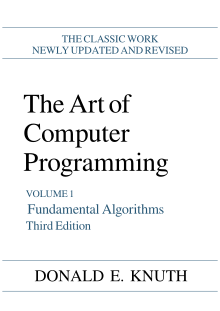
\includegraphics[width=0.2\linewidth]{img/chapter1/ArtOfComputerProgramming.png}
    \caption{Caption}
    \label{fig:book-1}
\end{figure}

\section{Goals}

Interdum et malesuada fames ac ante ipsum primis in faucibus. Suspendisse at vehicula nisi, ut tincidunt lacus. Donec nec enim metus. Morbi blandit, erat vitae pulvinar molestie, enim metus auctor elit, quis auctor nibh neque sit amet enim (Figure \ref{fig:book-1}). Maecenas vulputate dolor sit amet velit pharetra tempus. Aliquam ut lacinia nibh. Vestibulum tincidunt, neque id tincidunt placerat, lectus nisl eleifend libero, ut consequat risus neque a massa. Pellentesque vulputate, purus ut lobortis mollis, nulla sapien convallis erat, vitae gravida enim nisl ut mi. Maecenas et ipsum et enim commodo semper eget nec orci.

\section{Contributions}

In tincidunt tempor est ac feugiat. Pellentesque tempus, risus in dignissim sollicitudin, urna nisi hendrerit quam, a eleifend ligula mauris at lectus. Nulla quis massa magna. Ut volutpat accumsan enim, et cursus lectus imperdiet congue. Curabitur nec mi eget est congue tincidunt nec vel nunc. Sed lectus nunc, hendrerit a sollicitudin vitae, tempor at sapien. Ut consequat purus quis laoreet congue. Phasellus pulvinar velit at ultrices dapibus. Sed lacinia venenatis aliquet. Donec pharetra ipsum at ex rutrum commodo. Nulla pulvinar metus vel mi maximus maximus. Aenean eleifend at ligula sed feugiat. Cras id ante rhoncus, eleifend diam et, placerat ligula.
 % .tex extension is presumed
% \include{chapter2}
% \include{chapter3}
% \include{chapter4}
% \include{chapter5}


%%% Appendicies of thesis  %%%%%%%%%%%%%%%%%%%%%%%%%%%%%%%%%%%%%%%%%%%%%%%%%%%%%%%%%%%%%%%%%%%%%%%%

\appendix
% \include{appendixa}


%%% Bibliography  %%%%%%%%%%%%%%%%%%%%%%%%%%%%%%%%%%%%%%%%%%%%%%%%%%%%%%%%%%%%%%%%%%%%%%%%%%%%%%%%%

\printbibliography[title={References},heading=bibintoc]

% biblatex also supports chapter-by-chapter bibliography, https://tex.stackexchange.com/a/296502/119566
% see the biblatex manual, section 3.14.3


%%%% Option for natbib %%%%%%%%%%%%%

%%   use an appropriate style (.bst) and your own .bib file[s]

%\bibliographystyle{plainnat}
%\bibliography{mitthesis-sample.bib}

\end{document} 
 